\chapter{Model training}

\thispagestyle{empty}

\section{Random Forest algorithm}
\subsection{Decision Trees}
A decision tree is a type of supervised learning algorithms that is used for both classification and regression tasks. Decision trees learn a series of hierarchical `if/else` questions to classify data or predict outcomes.
\begin{figure}[h]
	\centering
	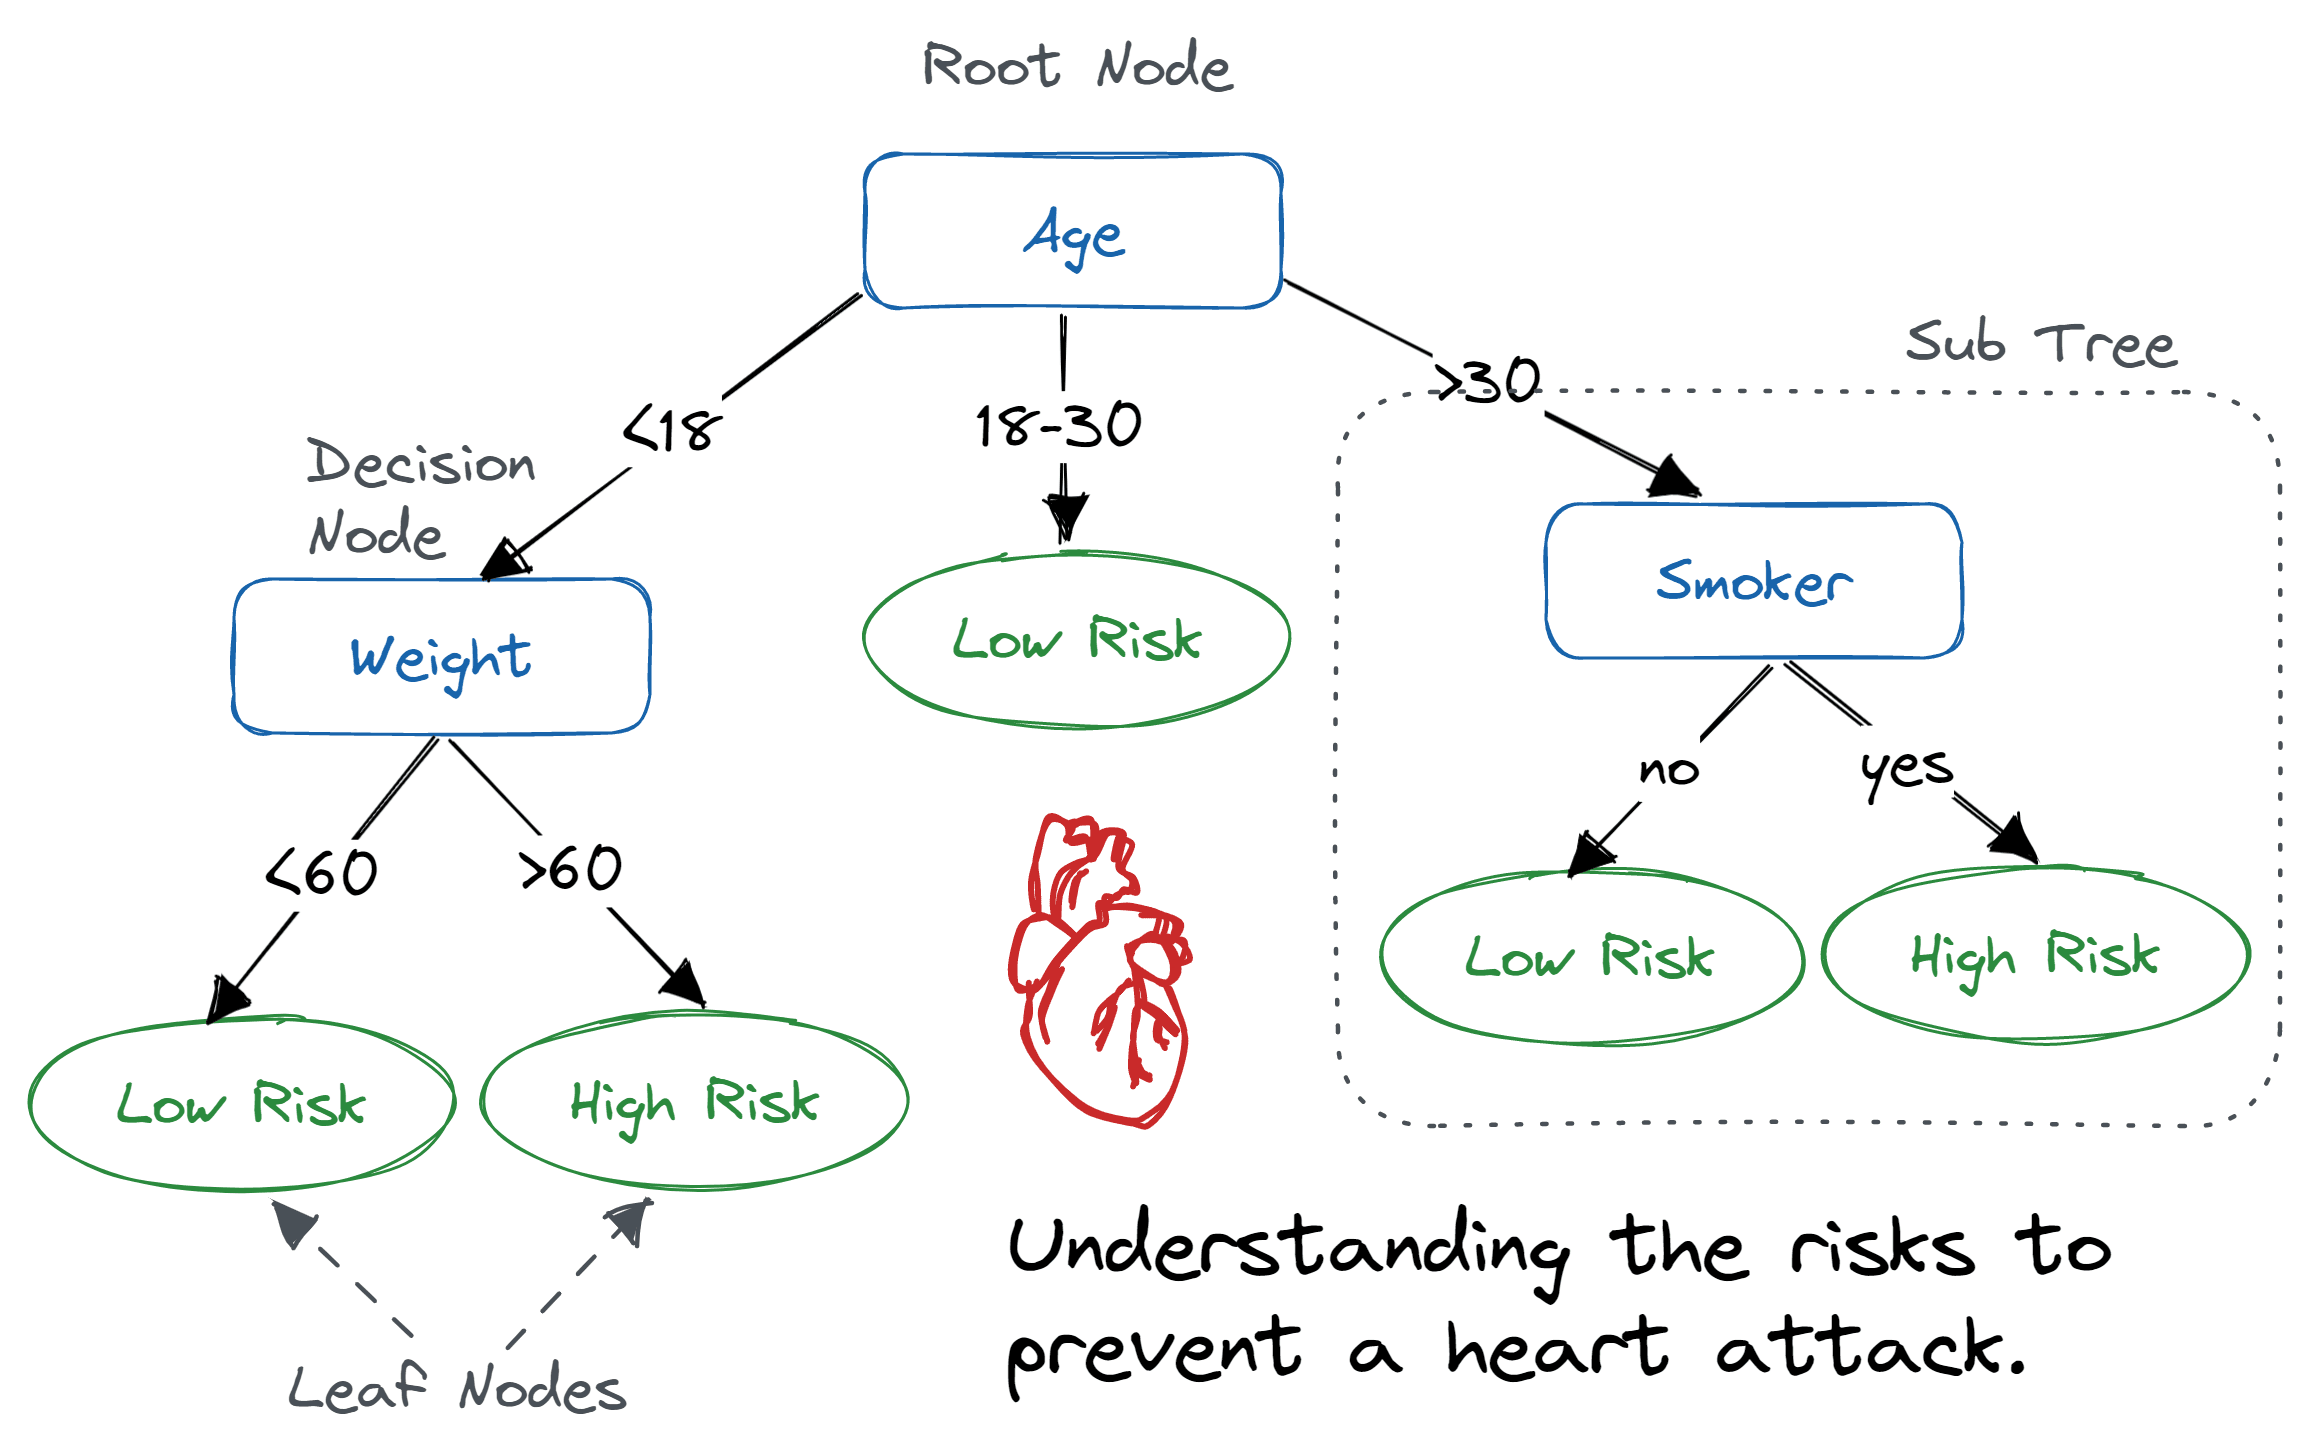
\includegraphics[width=0.9\textwidth]{./assets/images/decision_tree-examlpe.png}
	\caption{Decision Tree example}
\end{figure}

\subsection{Random Forests}
An ensemble learning method that uses a collection of decision trees to make predictions.

It builds multiple decision trees during training and outputs the class that is the mode of the classes (classification) or mean prediction (regression) of the individual trees.

\section{Feature extraction and engineering}

\section{Training the model}
